%% Header mit Deklarationen
\documentclass[%
enabledeprecatedfontcommands,
abstract=on,
paper=a4,      % alle weiteren Papierformat einstellbar
fontsize=11pt, % Schriftgr��e (12pt, 11pt (Standard))
BCOR1cm,       % Bindekorrektur, bspw. 1 cm
DIV15,         % f�hrt die Satzspiegelberechnung neu aus s. scrguide 2.4
oneside,       % Doppelseiten
headsepline,   %
headings=openright, % Kapitel nur rechts beginnen
%biblography=totoc, % Literaturverzeichnis einf�gen bibtotocnumbered: nummeriert
parskip=half,  % Europ�ischer Satz mit Abstand zwischen Abs�tzen
chapterprefix, % Kapitel anschreiben als Kapitel
headsepline,   % Linie nach Kopfzeile
titlepage,     %
numbers=noenddot,
%draft	       % zeigt �berlange Zeilen an
]{scrreprt}

\usepackage{units}
\usepackage{CTEX}
\usepackage{subfigure}
\usepackage{url} 
\usepackage{pdfpages}       % Titelseite hat ein anderes Layout. Sie wird 
                            % separat erzeugt und hier eingef�gt
\usepackage[utf8]{inputenc} % Zeichencodierung

\usepackage[ngerman, english]{babel} % Worttrennung nach neuer Rechtschreibung

\usepackage{ellipsis}       % Leerraum um Auslassungspunkte
\usepackage{fixltx2e}       % Fehlerkorrektur Zeichens�tze
\usepackage{xspace}         % f�ge evtl. notwendiges Leerzeichen hinzu (\xspace)

%\usepackage{mathptmx}           % Times + passende Mathefonts
\usepackage{mathpazo}           % Palatino + passende Mathefonts
\usepackage[scaled=.92]{helvet} % skalierte Helvetica als \sfdefault
\usepackage{courier}            % Courier als \ttdefault

\usepackage{graphicx}    % Einbindung von Grafiken
\graphicspath{{bilder/}} % Unterverzeichnis, in dem Grafiken abgelegt werden
\usepackage{listings}    % Listenausgabe externer Dateien

\usepackage{float}      % Paket zum Erweitern der Floatumgebungen
\usepackage[figuresright]{rotating}   % Rotieren von Objekten
%\usepackage{hvfloat}
\usepackage{array}      % Paket zum Erweitern der Tabelleneigenschaften
\usepackage{booktabs}   % Paket f�r sch�nere Tabellen

\usepackage{amsmath}    % erweiterte Mathematik-Umgebungen
\usepackage{amssymb}
\usepackage{esint}
% Einstellungen f�r das Literaturverzeichnis
\usepackage[colorlinks=true,linkcolor=blue,citecolor=blue,urlcolor=blue]{hyperref} % or backref
\usepackage[round]{natbib}
\setlength{\bibsep}{0.5\baselineskip}
\setlength{\bibhang}{1cm}
\bibliographystyle{agsm}

% Andere Schriftarten in Koma-Script
\setkomafont{sectioning}{\normalfont\bfseries}
\setkomafont{captionlabel}{\rmfamily\bfseries\small}
\setkomafont{caption}{\mdseries\itshape\small}
\setkomafont{pagehead}{\normalfont\itshape} % Kopfzeilenschrift
\setkomafont{descriptionlabel}{\normalfont\bfseries}

% Kopf und Fu�zeilen
\usepackage[automark]{scrlayer-scrpage}

% Literaturverzeichnis-Stil
%\bibliographystyle{plain}

% weitere Einstellungen
\tolerance=200               % �bervolle Zeile vermeiden
\emergencystretch=3em

\clubpenalty=10000           % 'Schusterjungen' und 'Hurenkinder' vermeiden
\widowpenalty=10000 
\displaywidowpenalty=10000

\parindent 0pt               % Einzug zu Absatzbeginn festlegen

\setcapindent{1em}           % Zeilenumbruch bei Bildbeschreibungen.

\setcounter{secnumdepth}{3}  % Strukturiertiefe bis subsubsection{} m�glich
\setcounter{tocdepth}{3}     % Dargestellte Strukturiertiefe im Inhaltsverzeichnis

% Korrekturversion mit 1.5-fachem Zeilenabstand im Hauptteil:
\newif\ifiscorrect
%\iscorrecttrue   % Korrekturversion
\iscorrectfalse % keine Korrekturversion

%% Eigene Definitionen:

% Einheiten:
\def\ut#1{\ensuremath{\,\mathrm{#1}}}

% Operatoren:
\def\grad{\ensuremath{\mathop{\mathrm{grad}}\nolimits}}
\def\transp#1{\ensuremath{{#1}^\mathsf{T}}}  % transpose
\def\const{\ensuremath{\mathop{\mathrm{const.}}\nolimits}}

% Formelzeichen:
\def\vec#1{\ensuremath{\mathbf{#1}}}
\def\matr#1{\ensuremath{\mathbf{#1}}}

% Hack, um ein zus�tzliches Leerzeichen nach \input zu entfernen:
\def\myinput#1{%
  \endlinechar=-1 % kein Zeilenabschlusszeichen
  \input #1\relax
  \endlinechar `\^^M % Zeilenabschluss = Zeilenvorschub
}


\begin{document}
	% R�mische Nummerierung f�r Sonderseiten, wie Verzeichnisse und Anhang
	\pagenumbering{Roman}
	\pagestyle{plain}
	
	%% Titelblatt
	%
\includepdf[pages=1]{extras/titelseite}
	
	
	% Inhalt Kopf-/Fu�zeile
	\pagestyle{scrheadings}
	\clearscrheadfoot            % Standardkram wegwerfen
	\ohead[\pagemark]{\pagemark} % oben au�en Seitenzahl 
	
	% Merke mir die r�mische Seitenzahl in 'roemisch' und setzte Nummeriernung 
	% auf arabisch f�r die eigentlichen Kapitel
	\cleardoublepage %\newpage
	\newcounter{roemisch}
	\setcounter{roemisch}{\value{page}}
	\pagenumbering{arabic}
	
	\ifiscorrect\linespread{1.5}\selectfont% Zeilenabstand: 1 1/2 (f�r bessere Korrektur)
	\else\fi
	
	%% Die einzelnen Kapitel
	% Kopfzeile: links Kapitel, rechts Sektion
	\clearscrheadfoot            % Standardkram wegwerfen
	\ohead[\pagemark]{\pagemark} % oben au�en Seitenzahl 
	\ihead{\headmark}            % oben innen automatischer Abschnittsname
	%\automark[]{section}
	\chapter{Segelbasierte Methoden}
\section{DE-ORBITING SATELLITES IN LEO USING SOLAR SAILS}
\subsection{Einführung und Motivation}
Die Beseitigung von Weltraumschrott ist zu einem sehr wichtigen Teil des kommerziellen und wissenschaftlichen Raumfahrtmanagements geworden. Besonders wichtig ist dies im erdnahen Orbit (Low Earth Orbit, LEO), wo es aufgrund der hohen Dichte an aktiven und inaktiven Satelliten wichtig ist, Zusammenstöße zwischen Raumfahrzeugen oder Teilen davon zu verhindern. 
\begin{figure}[htbp]
	\centering
	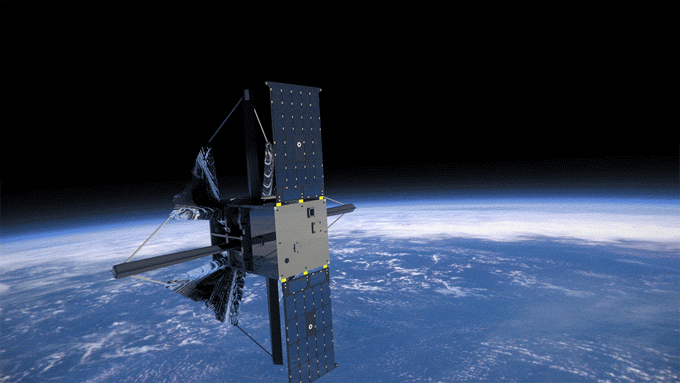
\includegraphics[width=0.7\textwidth]{bilder/Segel.png}
	\caption{Ein Bild, das zeigt, wie sich ein Sonnensegel in der Umlaufbahn um die Erde entfaltet. (Bildnachweis: NASA)}
	\label{Segel}
\end{figure}

Im Jahr 2006 unterzeichneten ASI, BNSC, CNES, DLR und ESA einen "Europäischen Verhaltenskodex", der eine Reihe von Vorschlägen enthält, wie die Zunahme von Weltraumschrott in den nächsten Jahren verhindert werden kann. Dieses Dokument führte im April 2008 zum ESA-Dokument "Requirements on Space Debris Mitigation for Agency Projects", das die Regeln festlegt, die von jeder zukünftigen europäischen Mission befolgt werden müssen. Nach diesen Regeln muss jeder europäische Satellit in einer Höhe von \unit[2000]{km} innerhalb von 25 Jahren nach dem Ende seiner Mission die Umlaufbahn verlassen. Mögliche Strategien bestehen darin, den Treibstoff an Bord zu nutzen, um am Ende der Lebensdauer des Raumfahrzeugs ein Wiedereintritt durchzuführen. Ein solcher Ansatz ist jedoch nicht durchführbar, wenn das Raumfahrzeug kein Antriebssystem an Bord hat. In diesem Fall muss eine alternative Lösung gefunden werden. Der auf Sonnensegeln basierende Ansatz erschien aus diesem Grund erstmals im Jahr 2011. \citet{Daniele:2012} erforschten den Einsatz von Sonnensegeln für das Deorbiting von Weltraumschrott. Abbildung \ref{Segel} zeigt wie sich ein Sonnensegel in der Umlaufbahn um die Erde entfaltet.


\subsection{Atmosphärischer Luftwiderstand}
Unter den verschiedenen Möglichkeiten und Konfigurationen stellt die Deorbitierung unter Nutzung des atmosphärischen Luftwiderstands und des solaren Strahlungsdrucks eine erste Anwendung dar. Der atmosphärische Luftwiderstand ist eine der Hauptquellen der störenden Beschleunigung für LEO-Satelliten. Diese Kraft $f_{drag}$ wird üblicherweise durch:
\begin{equation}
	\boldsymbol{f}_{\text {drag}}=-\frac{1}{2} C_D \rho(\boldsymbol{r}, t) \frac{A}{m}\left(\boldsymbol{V}-\boldsymbol{V}_{a t m}\right) \mid\boldsymbol{V}-\boldsymbol{V}_{a t m} \mid
	\label{Luftreibung}
\end{equation}
beschrieben, mit dem Widerstandsbeiwert $C_D$, der Dichte der Atmosphäre $\rho$, dem Fläche-Masse-Verhältnis $\frac{A}{m}$, der Geschwindigkeit des Raumfahrzeugs $\boldsymbol{V}$ und der Geschwindigkeit der Atmosphäre $\boldsymbol{V}_{a t m}$.

Der Luftwiderstand hängt von vielen Faktoren ab, und es ist leicht zu erkennen, dass er erhöht werden kann, wenn der Wert vom Fläche-Masse-Verhältnis erhöht wird, und somit die Zeit von Deorbiting verkürzt werden kann. Der Einsatz von Sonnensegeln als Aerobraking-Geräte gegen Weltraumschrott und zur Reduzierung der Anzahl potenziell gefährlicher Objekte in der niedrigen Erdumlaufbahn ist deswegen eine Anwendung. Es ist möglich, den Wert vom Fläche-Masse-Verhältnis mit Hilfe eines Sonnensegels zu erhöhen und so das Deorbiting zu beschleunigen.

\subsection{Gossamer Projekt}
Das Deutsche Zentrum für Luft- und Raumfahrt (DLR) war eines der ersten Forschungszentren, das sich mit der Technologie der Sonnensegel befasst hat. Tatsächlich hat das DLR bereits im Jahr 1999 einen erfolgreichen Test zur Entwicklung eines $20\times20$ Meter großen Segels durchgeführt. Im Jahr 2010 wurden die Solarsegel-Aktivitäten wieder aufgenommen und das von der ESA geförderte Gossamer-Projekt, wurde auf dem $2^{nd}$ International Symposium on Solar Sailing in New York offiziell vorgestellt \citep{Geppert:2011}. Die im Rahmen des ESA-Projekts "Deployable Gossamer Sail for Deorbiting" durchgeführte Aktivität konzentrierte sich auf die die Reduzierung von Weltraumschrott in der LEO-Orbit. Die Aktivität bestand in der Entwicklung eines End-of-Life-Debitsystems, dem sogenannten Gossamer Deorbiter, der es neuen Raumfahrzeugen ermöglichen wird, den Europäischen Verhaltenskodex zu erfüllen \citep{FERNANDEZ:2014}.

Der erste Schritt des Gossamer-Projekts ist der Einsatz eines $5\times5$ Meter großen Sonnensegels in der Erdumlaufbahn, um die Möglichkeiten der Herstellung, der Verpackung und des erfolgreichen Einsatzes eines vollständig Systems im Weltraum zu beweisen. Die Weiterentwicklung von Gossamer-2 besteht darin, in der Erdumlaufbahn eine vorläufige Lage- und Bahnregelung zu testen. Als dritter Schritt des Programms, Gossamer-3, ist schließlich eine interplanetare Mission in vollem Umfang geplant. 

\subsection{Vorbereitung auf die Simulation}
Um die Möglichkeit des Einsatzes von Sonnensegeln zu untersuchen, wurden Simulationen in Matlab durchgeführt und die Ergebnisse mit denen aus dem Papier von \citet{Daniele:2012} verglichen. 

Die Untersuchung der Auswirkungen des atmosphärischen Luftwiderstands auf ein Raumfahrzeug ist eine der größten Herausforderungen bei der Simulation. Von den bereits erwähnten Harris–Priester - und MSIS-Modellen ist das MSIS-Modell zwar genauer, aber aufgrund des riesigen Zeitaufwands mussten wir es zugunsten des effizienteren Harris–Prieste Modells aufgeben. Auf dieser Grundlage wurden die Keplerschen Elemente der Satellitenbahn in Matlab simuliert, wobei ODE113 zur Integration verwendet wurde. 

Neben der Umlaufbahn des Satelliten beeinflusst die Attitude des Sonnensegels den Luftwiderstand. Aufgrund der Komplexität der Attitude-lösung haben wir dies in den Matlab-Simulationen jedoch nicht berücksichtigt, sondern sind davon ausgegangen, dass die Orientierung des Sonnensegels zu jedem Zeitpunkt konstant ist, was natürlich nicht der Realität entspricht. In gewisser Weise gehen wir davon aus, dass das aerodynamische Drehmoment stark genug ist, um eine passive Stabilisierung zu gewährleisten, wie wir später noch genauer erläutern werden. 

Unser Testszenario berücksichtigt die folgenden Bedingungen:
\begin{itemize}
	\item Orbit: \unit[600]{km} Höhe
	\item Gesamtmasse des Satelliten: \unit[2500]{kg} / \unit[500]{kg}
	\item Segelfläche: \unit[25]{$m^2$}
\end{itemize}
\clearpage
\subsection{Analyse der Ergebnisse}
\begin{figure}[htbp]
	\centering
	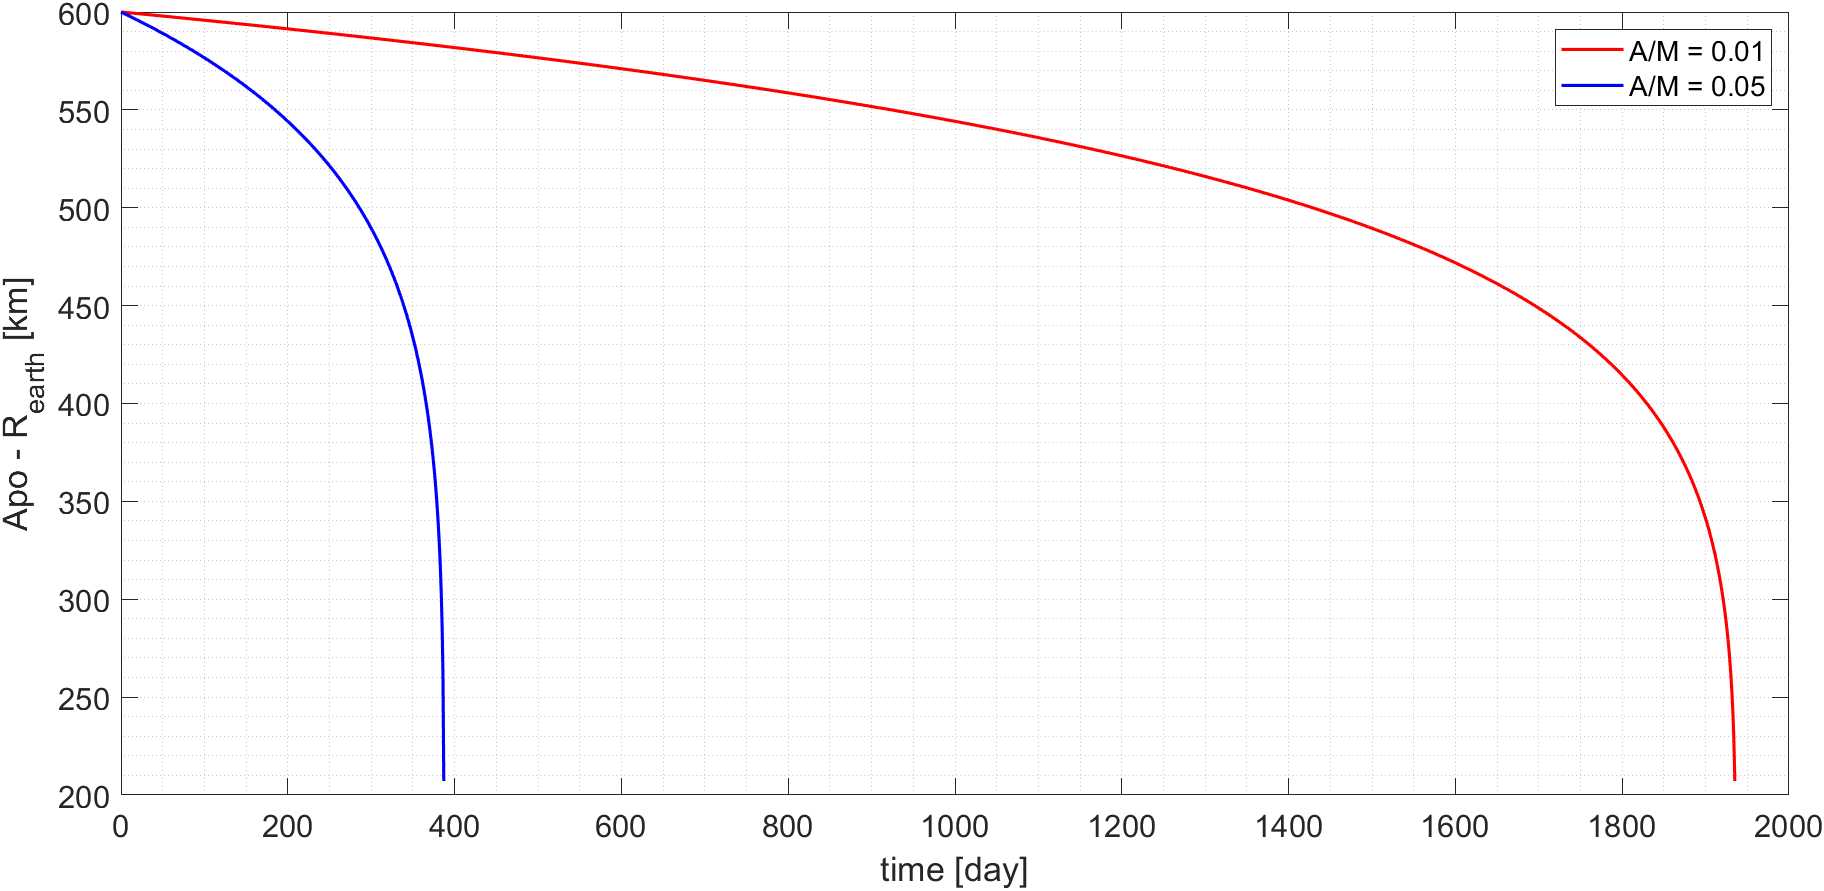
\includegraphics[width=0.7\textwidth]{bilder/Simulation_Matlab.png}
	\caption{Ergebnisse der Simulation in Matlab: Änderung der Höhe des Apogäums mit der Zeit nach Abzug des Erdradius, wobei rot das Ergebnis eines A/M von 0,01 und blau das Ergebnis eines A/M von 0,05 ist.}
	\label{Simulation_Matlab}
\end{figure}
Die Ergebnisse der Simulation in Matlab sind in Abbildung \ref{Simulation_Matlab} dargestellt. Wir haben zwei verschiedene A/M ausprobiert, die mit ODE113 berechnet wurden, um die Veränderung der Apogäumshöhe über die Zeit nach Abzug des Erdradius zu ermitteln. Die Simulation zeigt, dass das Raumfahrzeug im Testszenario mit A/M = 0,05 in etwa \unit[2000]{Tagen} wieder in die Atmosphäre eintritt: Es ist zu beachten, dass der Satellit als wieder in die Atmosphäre eingetreten gilt, wenn es eine Höhe von \unit[150]{km} über dem Geoid erreicht. Das ist sicherlich nicht ideal, aber wenn das A/M um den Faktor fünf erhöht wird, verkürzt sich die Zeit signifikant auch um einen Faktor von fast fünf.

\begin{figure}[htbp]
	\centering
	\includegraphics[width=0.6\textwidth]{bilder/Simulation_paper.png}
	\caption{Höhe des Satelliten über dem Geoid im Laufe der Zeit mit einer Orbithöhe von \unit[450]{km},  Gesamtmasse von \unit[140]{kg} und einer Segelfläche von \unit[25]{$m^2$}}
	\label{Simulation_paper}
\end{figure}
\clearpage
Das erste Testszenario in dem Papier verwendet unterschiedliche Bedingungen: 
\begin{itemize}
	\item Orbit: \unit[450]{km} Höhe
	\item Gesamtmasse des Satelliten: \unit[140 ]{kg}
	\item Segelfläche: \unit[25]{$m^2$}
\end{itemize}
Abbildung \ref{Simulation_paper} zeigt nicht die Apogäumshöhe, sondern die Bahnhöhe, und die Schwankungen im Bild sind auch auf die elliptische Bahn zurückzuführen. Obwohl die Szenarien unterschiedlich sind, zeigen unsere Simulationsergebnisse und die Ergebnisse im Papier ähnliche Trends. Mit einem A/M von ca. 0,18 wurde die Bahnhöhe in nur 20 Tagen von 450 km auf 150 km reduziert. Die vorläufigen Schlussfolgerung ist, dass die Verwendung eines Sonnensegels kann daher nützlich sein. 

Weitere Untersuchungen müssen jedoch in einem allgemeineren Rahmen durchgeführt werden, um festzustellen, in welcher Höhe die Ausleger des Sonnensegels nicht mehr in der Lage sind, die aerodynamischen Drehmomente zu bewältigen, was zum Zusammenbruch der Struktur führt. Wie bereits erwähnt, ist die Ausrichtung des Sonnensegels entscheidend, denn eine stabile Orientierung ist notwendig, um eine stabile Querschnittsfläche und den Luftwiderstand zu gewährleisten, was in unseren Simulationen nicht berücksichtigt wird. Da in das Papier wurde die Attitude des Sonnensegels zusammen mit der Bahnbewegung berücksichtigt, ist es möglich, den Querschnitt in Bezug auf die Atmosphäre über die Zeit während der Simulation darzustellen (Siehe Abbildung \ref{Attitude_Paper}).
\begin{figure}[htbp]
	\centering
	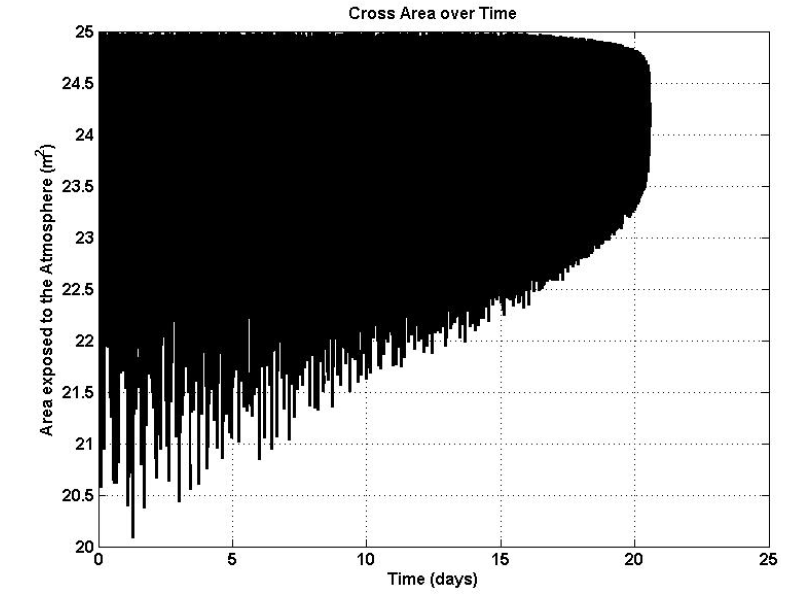
\includegraphics[width=0.7\textwidth]{bilder/Attitude_Paper.png}
	\caption{Querschnittsfläche über die Zeit}
	\label{Attitude_Paper}
\end{figure}
\clearpage
Es ist klar, dass das aerodynamische Drehmoment, das auf dem Sonnensegel wirkt, stark genug ist, um eine passive Stabilisierung zu gewährleisten, wobei das Segel wie ein Fallschirm wirkt und der verdünnten Atmosphäre eine konstante Fläche von etwa \unit[24]{$m^2$} bietet. Aufgrund des aerodynamischen Drehmoments wird der Luftwiderstand des Segels kostenlos maximiert ohne eine aktive Steuerung. Es ist aber wichtig zu beachten, dass diese passive Stabilisierung nur erreicht werden kann, wenn das aerodynamische Drehmoment stark genug ist. 
\begin{figure}[htbp]
	\centering
	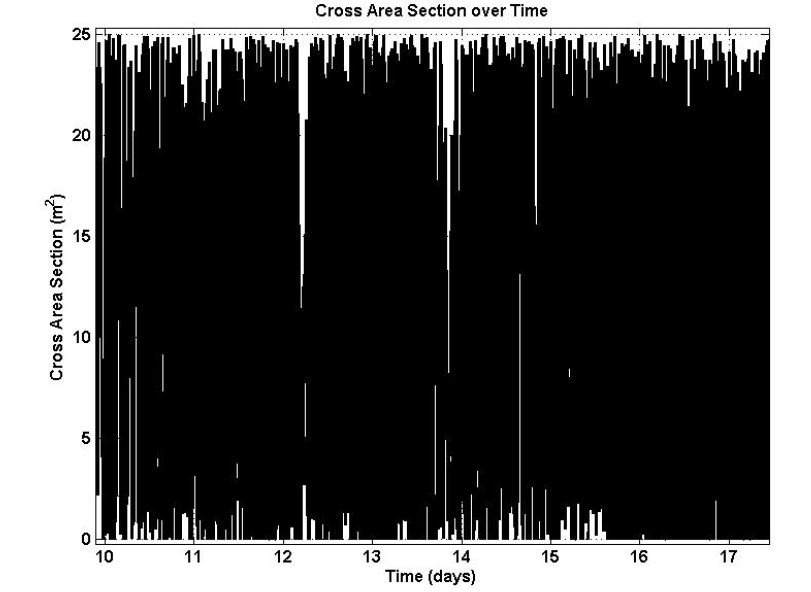
\includegraphics[width=0.7\textwidth]{bilder/Attitude2_Paper.png}
	\caption{Querschnitt über die Zeit (detaillierte Ansicht eines Zeitraums von einer Woche) mit einer Bahnhöhe von \unit[600]{km},  Gesamtmasse von \unit[140]{kg} und einer Segelfläche von \unit[25]{$m^2$}}
	\label{Attitude2_Paper}
\end{figure}

Die Situation wird nicht optimal, wenn die Bahnhöhe ansteigt. Neue Simulationen mit einer Bahnhöhe von \unit[600]{km} zeigt, dass die gewünschte "passive Stabilisierung" zur Maximierung der Fläche kann nicht mehr erreicht werden. Das liegt daran, dass das verfügbare aerodynamische Drehmoment nicht ausreicht, um die Rotation des Satelliten auszugleichen. Tatsächlich ist die atmosphärische Dichte in \unit[600]{$km$} Höhe um ein bis zwei Größenordnungen geringer als in \unit[450]{$km$} km Höhe, was gemäß Gleichung \ref{Luftreibung} zu einer viel geringeren Widerstandskraft führt. Das bedeutet, dass die Situation, die wir in Matlab simulieren, in der Realität nicht realisierbar ist. In Abbildung \ref{Attitude2_Paper} ist es zu sehen, dass der Satellit erheblich taumelt, was zu einer Querschnittsfläche im gesamten Bereich zwischen \unit[0]{$m^2$} und \unit[25]{$m^2$} führt.

\subsection{Zusammenfassung}
In diesem Abschnitt wurde die Möglichkeit untersucht, ein Sonnensegel für das Deorbiting in der LEO-Orbit zu verwenden. Es wurden die theoretischen Grundlagen für die Simulation einer solchen Anwendung erläutert und die wichtigsten Probleme beschrieben, die bei dieser Aufgabe auftreten können. Die vorläufige Analyse hat gezeigt, dass die Verwendung eines Sonnensegels unter bestimmten Einschränkungen nützlich sein. Für die Realisierung dieses Verfahrens sind natürlich detailliertere Versuchsdaten erforderlich.


\section{DE-ORBITING SATELLITES IN LEO USING SOLAR SAILS}
\subsection{Einführung}
Der solare Strahlungsdruck ist die Störung, die durch die Wechselwirkung zwischen den von der Sonne kommenden Photonen und der äußeren Oberfläche des Satelliten entsteht. Obwohl Sonnensegel auf solche Wechselwirkungen angewiesen sind, um Schub zu erzeugen, ist diese Wechselwirkung eine Störung für Satelliten in der LEO-Orbit und haben um mehrere Größenordnungen weniger Wirkung als andere. Für höhere Umlaufbahnen, wie z.B. geosynchrone Umlaufbahnen, bietet der solare Strahlungsdruck aber eine einzigartige Lösung, um größeren Weltraumschrott zu entfernen. 

Nach dem aktuellen Stand der Technik kann ein CubeSat mit einem Hochleistungs-Sonnensegel als Antrieb Satelliten in der Größenordnung von \unit[1000]{kg} deorbitieren. Dieser CubeSat, auch "TugSat" genannt, wird in der Studie  von \citet{Kelly:2018} simuliert und einen Satelliten virtuell aus der geostationären Umlaufbahn ohne den Einsatz von Standard-Antriebssystemen deorbittet. Dieser TugSat kann zwischen dem geostationären Orbit und dem Friedhofsorbit wiederverwendet werden, um kontinuierlich Schrott aus den wertvollen geostationären Umlaufbahn zu entfernen. Das gesamte Deorbit-Manöver wird die Kontrolle über die Halbachse des Sateliten, die Exzentrizität, die Inklination darstellen: alles unter Verwendung von Techniken zur Optimierung der zeitlichen Änderungsraten der Bahnelemente des Satelliten. 
\subsection{Kraft aufgrund von Solardruck}
Die Formel für die Kraft, die durch den Strahlungsdruck der Sonne entsteht, lautet wie folgt:
\begin{equation}
	\boldsymbol{f}=-\kappa P_{\odot} \frac{A U^2}{r_{\odot}^2} \frac{A}{m} \cos \theta\left[(1-\varepsilon) \hat{\boldsymbol{r}}_{\odot}+2 \varepsilon \cos \theta ~\widehat{\boldsymbol{n}}\right]
\end{equation}
\begin{itemize}
	\item $P_{\odot}$: Größenordnung des solaren Strahlungsdrucks
	\item $r_{\odot}$: die Distanz zum Satelliten
	\item $AU$: die astronomische Einheit
	\item $\kappa$: der Schattenkoeffizient
	\item $\epsilon$: der Reflexionskoeffizient
	\item $\frac{A}{m}$: das Flächen-Masse-Verhältnis
	\item Winkel $\theta$ zwischen dem Sonnenrichtungsvektor $\hat{\boldsymbol{r}}_{\odot}$ und der Segelflächennormale $\widehat{n}$
\end{itemize}
Unter einigen Annahmen, ${AU}^2\approx1,~\kappa=1,~\epsilon=1$, kann eine charakteristische Kraft definiert werden als: 
\begin{equation}
	\ddot{\boldsymbol{r}}_{\mathrm{SRP}} \approx-a_c \cos ^2 \theta ~\hat{\boldsymbol{n}}, \quad \theta \in\left[0, \frac{\pi}{2}\right]
	\label{SRP}
\end{equation}
Aus Gleichung \ref{SRP} geht hervor, dass die Größe des solaren Strahlungsdrucks direkt von der Richtung der Normalen der Segeloberfläche abhängt. 

Die Simulation basiert auf einem \unit[50]{kg} schweren Satelliten, der mit einem perfekt reflektierenden, \unit[800]{$m^2$} (ca. 28 $\times$ \unit[28]{$m^2$} ) großen Sonnensegel ausgestattet ist. Mit der zusätzlichen Masse einer \unit[1000]{kg} schweren Nutzlast beträgt das Flächen-Masse-Verhältnis des Gesamtsystems \unit[0,76]{$m^2 / kg$}.

\subsection{TugSat}
Die TugSat-Simulation soll das Potenzial zeigen, mit einem Sonnensegelsatelliten Weltraumschrott aus dem GEO-Orbit zu entfernen. TugSat wird in einer  Umlaufbahn innerhalb des GEO-Orbits gestartet und beginnt damit, die Hauptachse seiner Umlaufbahn um \unit[350]{km} anzuheben. Sobald das Ziel der semimajoralen Achse erreicht ist, wird TugSat die Exzentrizität seiner neuen Umlaufbahn verringern und dabei eine Höhe für Friedhofsumlaufbahnen beibehalten. Als Nächstes lässt TugSat die Nutzlast los und beginnt mit dem Abstieg zurück in den GEO-Orbit.
Diese Manöver werden unter Verwendung der optimierten Segelausrichtung durchgeführt.
\subsection{Simulation}
Nachdem die primären Manöver beschrieben wurden, kann die gesamte TugSat-Simulation dargestellt werden. 
Das erste Ziel beim Deorbit mit TugSat ist es, die Hauptachse der Nutzlast zu vergrößern. TugSat wird die Nutzlast deorbitieren, indem es das Apogäum erhöht und die Halbachse \unit[350]{km} über dem GEO-Orbit anhebt. Sobald die gewünschte Halbachse erreicht ist, verringert TugSat die Exzentrizität der Umlaufbahn, bevor es die Nutzlast freilässt. Nach der Freigabe der Nutzlast kehrt Tugsat in den GEO-Orbit zurück und peilt seine ursprüngliche Länge vom Beginn der Simulation an. Abbildung \ref{Simulation_TugSat} zeigt die TugSat-Simulation. TugSat deorbiert erfolgreich und lässt seine Nutzlast in weniger als einem Jahr frei. In weniger als anderthalb Jahren kehrt TugSat erfolgreich zum GEO-Orbit zurück. In weniger als zwei Jahren nach Beginn des Deorbit-Manövers reduziert TugSat die Bewegung auf weniger als \unit[5]{km}, während die Werte für die Hauptachse, die Exzentrizität konstant bleiben.

\begin{figure}[htbp]
	\centering
	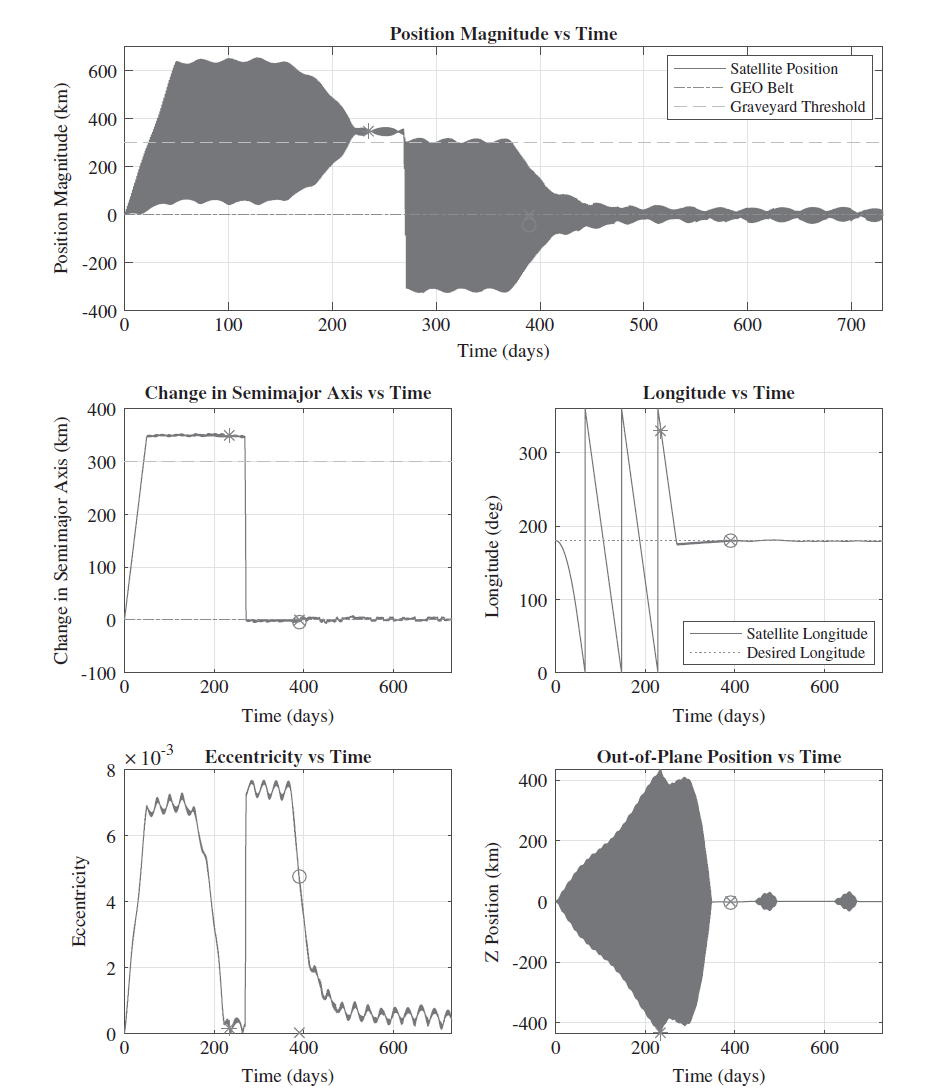
\includegraphics[width=0.8\textwidth]{bilder/Simulation_TugSat.png}
	\caption{TugSat-Simulationsergebnisse: Der Stern steht für die Freigabe der Nutzlast}
	\label{Simulation_TugSat}
\end{figure}

\subsection{Zusammenfassung}
Der solare Strahlungsdruck ist eine wichtige Ressource für Satelliten in hoch gelegenen Umlaufbahnen, insbesondere in der geostationären Umlaufbahn, und bietet eine Möglichkeit für niedrigpräzise, unbegrenzte Satellitenmanöver. Es ist noch mehr Forschung nötig, um diese Idee in Zukunft tatsächlich umzusetzen.

\chapter{Statistische Analyse}
\begin{figure}[htbp]
	\centering
	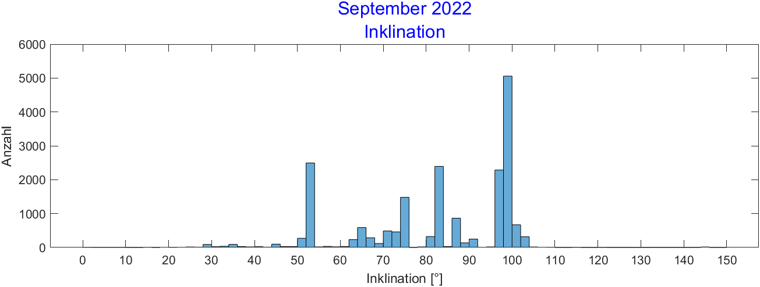
\includegraphics[width=1\textwidth]{bilder/Inklination.png}
	\caption{Screenshot des in der Präsentation gezeigten GIF: die Inklination aller Objekte im LEO-Orbit von von 2005 bis 2022}
	\label{Inklination}
\end{figure}
Die Inklination eines Satelliten ist eng mit seiner Nutzung verbunden. In Abbildung \ref{Inklination} ist leicht zu erkennen, dass die Inklination der meisten Objekte zwischen 50° und 110° liegt. Davon befinden sich Satelliten mit einer Inklination von etwa 100° wahrscheinlich in einer sonnensynchronen Umlaufbahn, während eine Inklination von 63,4° wird oft als kritische Inklination bezeichnet, weil sie keine Apogäumsdrift haben.
\clearpage
\begin{figure}[htbp]
	\centering
	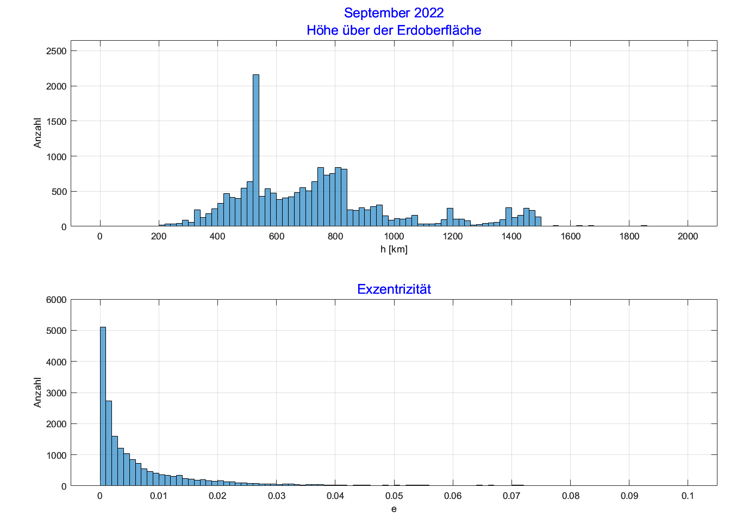
\includegraphics[width=1\textwidth]{bilder/Hoehe.png}
	\caption{Screenshot des in der Präsentation gezeigten GIF: die Inklination aller Objekte im LEO-Orbit von von 2005 bis 2022}
	\label{Hoehe}
\end{figure}
Abbildung \ref{Hoehe} zeigt die Verteilung der Exzentrizität und Höhe aller Objekte im LEO-Orbit. Fast alle Objekte sind zwischen \unit[200]{km} und \unit[1600]{km} konzentriert und haben eine sehr geringe Exzentrizität. Das bedeutet auch, dass dieses Gebiet mit extrem dichten Objekten mit Weltraummüll gefüllt ist, was einen erheblichen negativen Einfluss auf die Funktionsfähigkeit von Satelliten hat.
\clearpage
\begin{figure}[htbp]
	\centering
	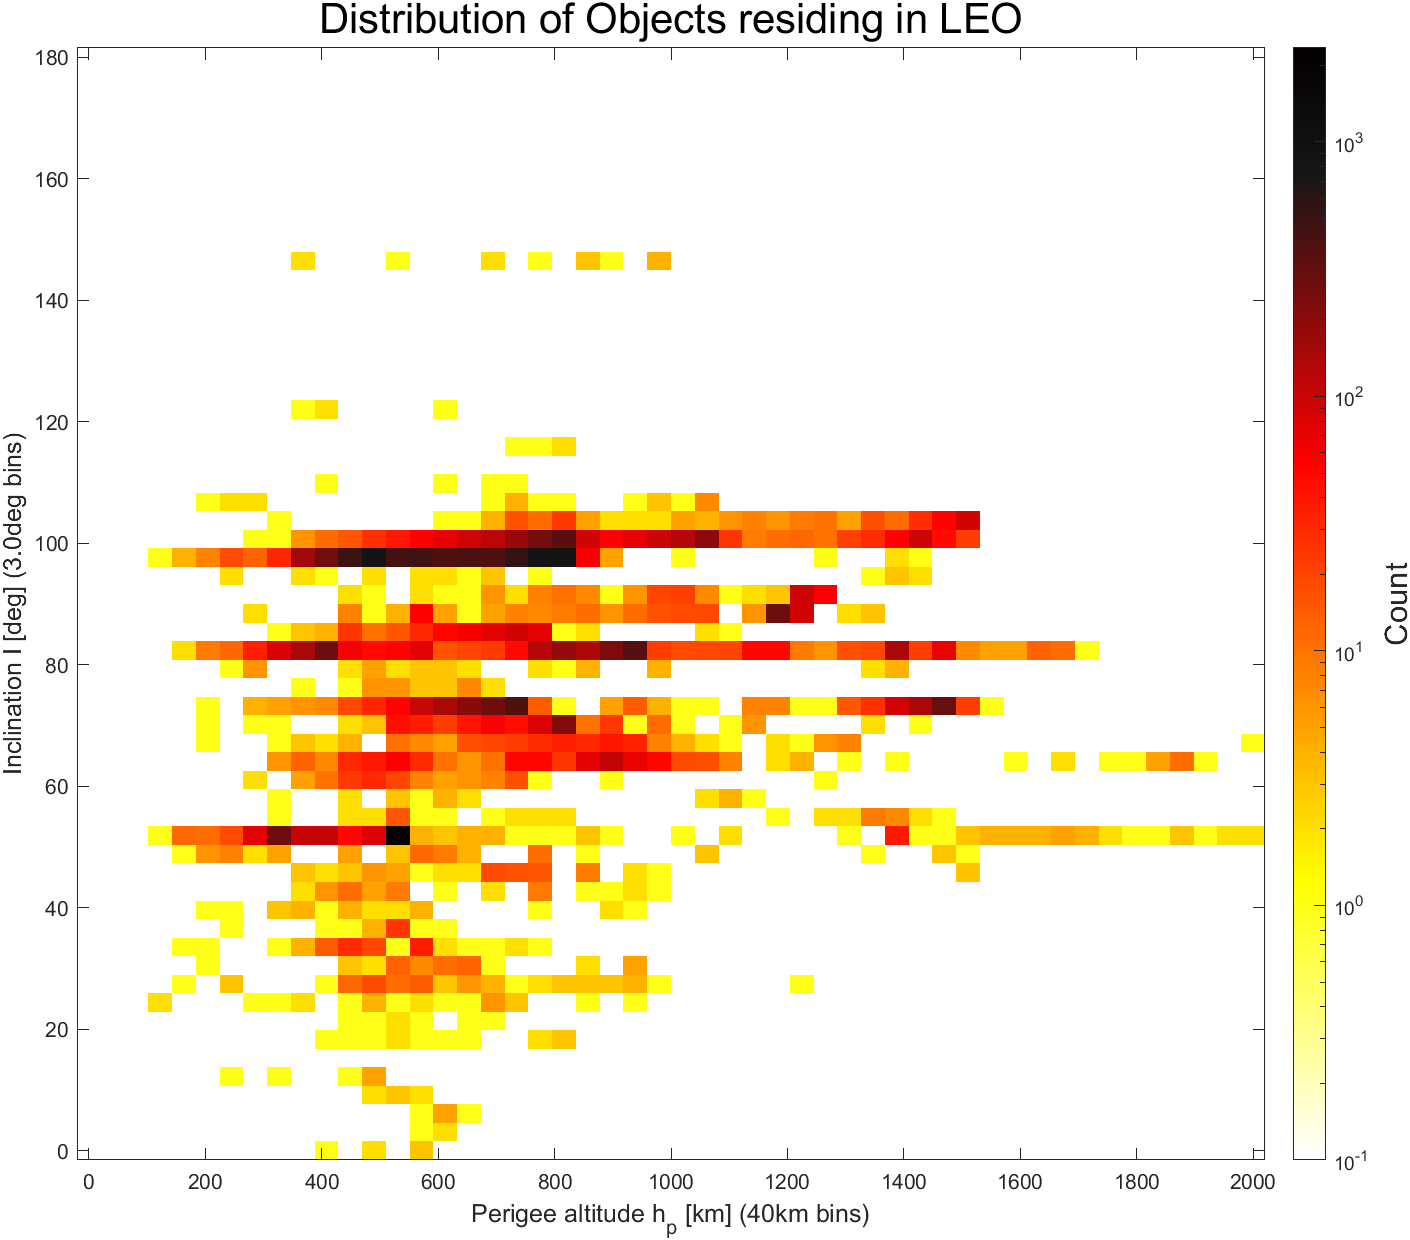
\includegraphics[width=0.5\textwidth]{bilder/Distribution_1.png}
	\caption{Verteilung der Anzahl der Objekte im LEO als Funktion der Inklination und der Perigäumshöhe.}
	\label{Distribution_1}
\end{figure}

\begin{figure}[htbp]
	\centering
	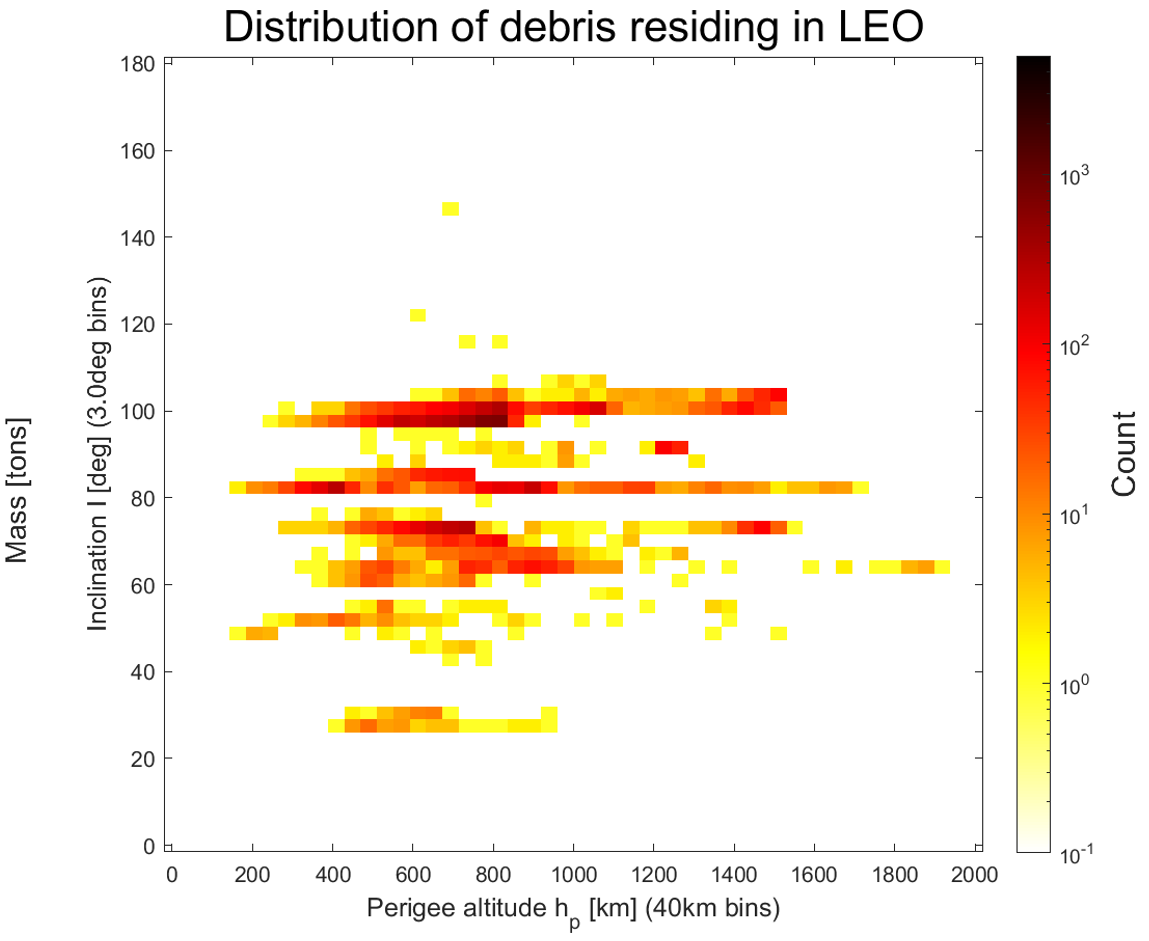
\includegraphics[width=0.6\textwidth]{bilder/Distribution_2.png}
	\caption{Verteilung der Anzahl der space debris im LEO als Funktion der Inklination und der Perigäumshöhe.}
	\label{Distribution_2}
\end{figure}
Abbildung \ref{Distribution_1}, \ref{Distribution_2} zeigen die Verteilung aller Objekte und des Weltraumschrotts in der LEO-Orbit in einem zweidimensionalen Histogramm. Die Perigäumshöhe wird in \unit[40]{km}-Bins gezählt, während die Inklination in 3°-Bins gezählt wird. Der Vergleich zeigt, dass Gebiete mit einer hohen Dichte an Objekten auch eine große Menge an Weltraumschrott haben. Zum Beispiel gibt es mehrere tausend Objekte in einem Gebiet mit einer Höhe von 400-600 km und einer Inklination von etwa 100°. Gleichzeitig kann auch festgestellt werden, dass sich fast tausend Weltraumschrott im selben Gebiet versammelt haben, was sehr gefährlich ist.

	\bibliography{literatur/bib}
\end{document}